\section{Pendahuluan}
\subsection{Latar Belakang}
Bagian ini menjelaskan alasan dilaksanakannya praktikum, termasuk pentingnya topik yang dibahas. Latar belakang mencantumkan permasalahan yang ingin diselesaikan, urgensi pembelajaran topik, serta keterkaitannya dengan aplikasi dunia nyata atau teknologi saat ini.

\subsection{Dasar Teori}
Bagian ini memuat teori-teori dasar yang mendukung pelaksanaan praktikum. Penjelasan mencakup konsep teknis, nama istilah, serta prinsip ilmiah yang relevan. Tujuannya adalah untuk memberikan pemahaman mendalam sebelum praktikum dilakukan.

%===========================================================%
\section{Tugas Pendahuluan}
Bagian ini berisi jawaban dari tugas pendahuluan yang telah anda kerjakan, beserta penjelasan dari jawaban tersebut
\begin{enumerate}
	\item Karena ada empat departemen yang berbeda, maka kita perlu 
	menggunakan empat subnet yang berbeda untuk masing-masing 
	departemen. Besar subnet yang dibutuhkan dapat dihitung 
	dengan menambah dua pada banyak perangkat dan membulatkan 
	ke atas ke pangkat 2 terdekat.
	{\small
		\begin{center}
		\begin{tabular}{ |c|c|c|c|c|c|c| } 
			\hline
			Departemen & Perangkat & Host yang dibutuhkan & Besar subnet & CIDR & Banyak host & Subnet Address \\
			\hline
			RnD & 100 & $ \geq $ 102 & /25 & /25 & 126 & 192.168.0.0/25 \\
			Produksi & 50 & $ \geq $ 52 & /26 & /26 & 62 & 192.168.0.128/26 \\
			Administrasi & 20 & $ \geq $ 22 & /27 & /27 & 30 & 192.168.0.192/27 \\
			Keuangan & 10 & $ \geq $ 12 & /28 & /28 & 14 & 192.168.0.0/28 \\
			\hline
		\end{tabular}
		\end{center}
	}
	Dapat dilihat bahwa CIDR yang digunakan adalah /25, /26, /27, dan /28.
	Banyak host yang dapat digunakan pada masing-masing subnet adalah 126, 
	62, 30, dan 14. Hal ini karena dua host telah digunakan untuk network 
	address (host pertama) dan broadcast address (host terakhir).
	\item Karena semua perangkat menuju ke satu router, 
	maka bentuk topologi yang terbentuk adalah topologi star.
	\begin{center}
		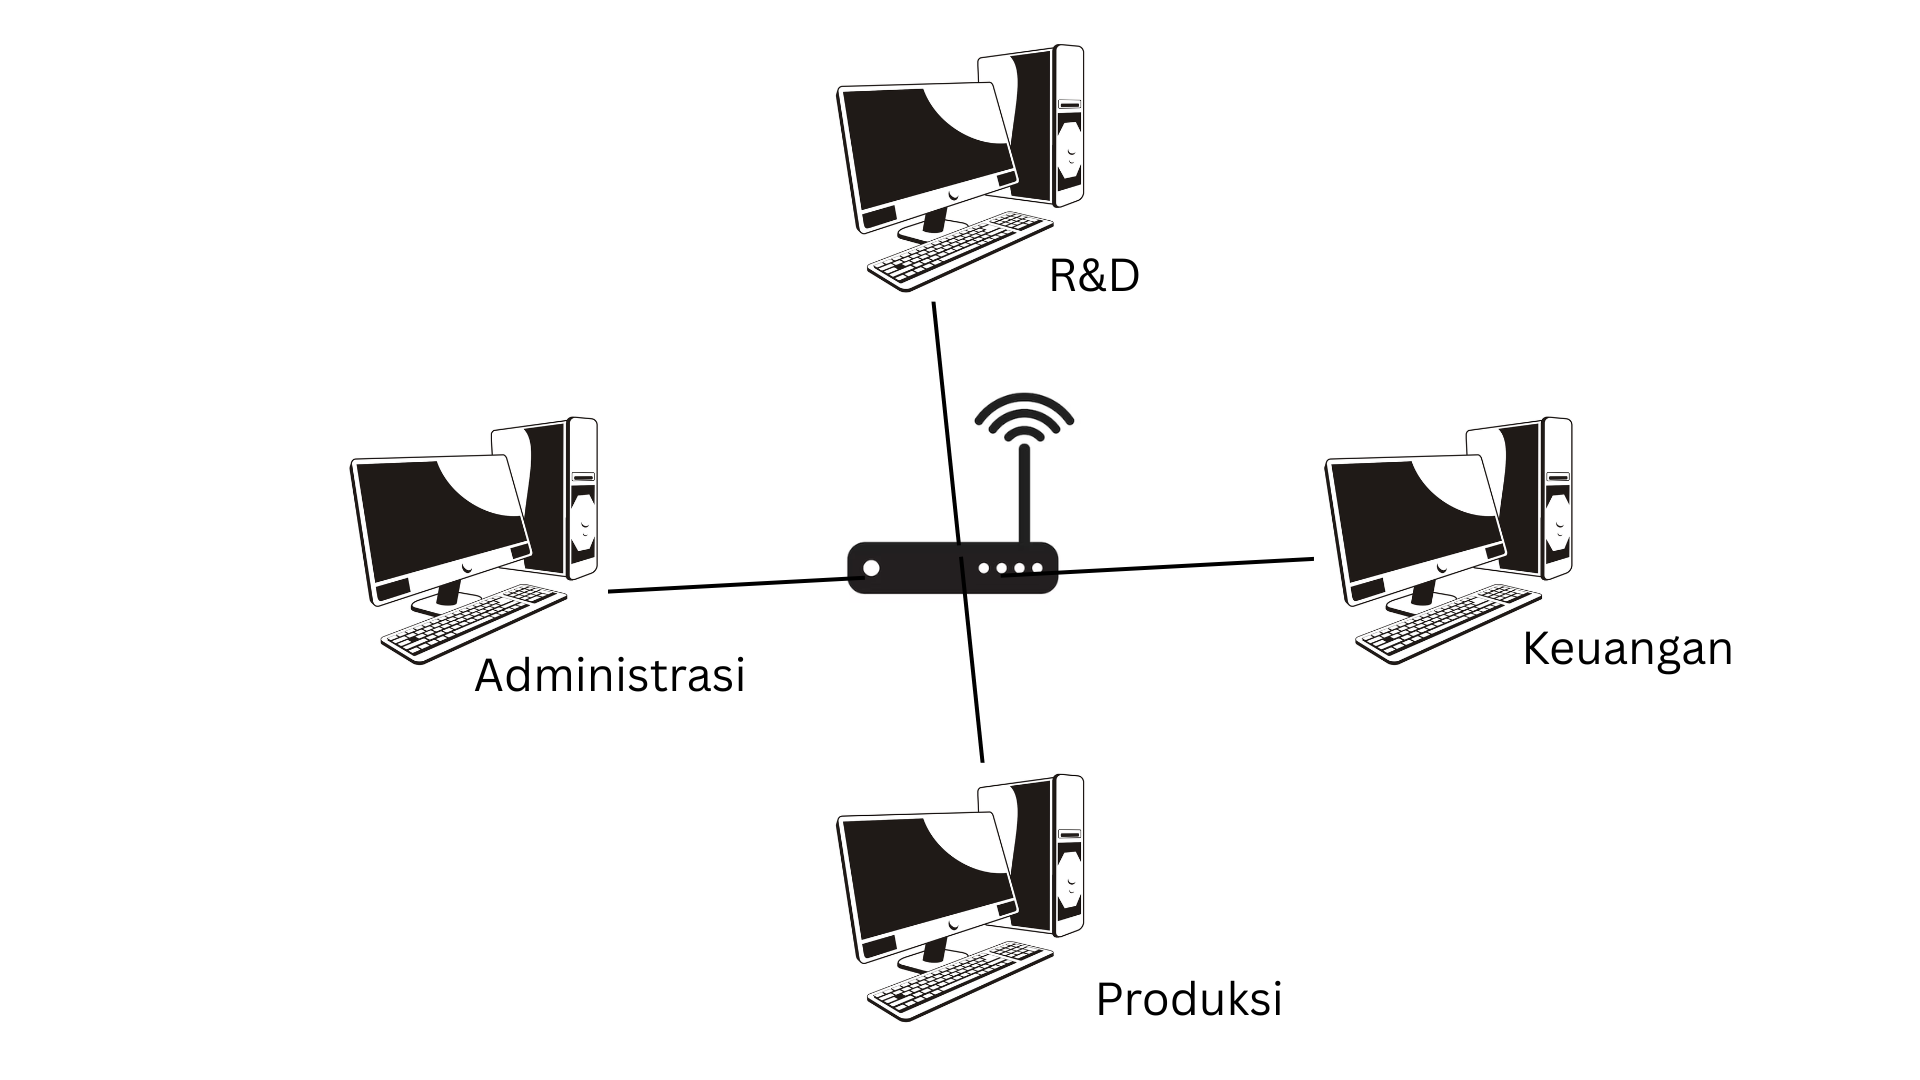
\includegraphics[scale=0.22]{P1/img/topology.png}
    \end{center}
	\item Berikut tabel routing sederhana. Karena semua perangkat 
	terhubung ke satu router tanpa perantara, maka tidak diperlukkan 
	gateway. Sedangkan interface menunjukkan kemana pengiriman 
	paket untuk masing-masing subnet.
	{\small
		\begin{center}
		\begin{tabular}{ |c|c|c|c| } 
			\hline
			Destinasi Network & Netmask/prefix & Gateway & Interface \\
			\hline
			192.168.0.0 & /25 & --- & RnD (eth0)  \\
			192.168.0.128 & /26 & --- & Produksi (eth1)  \\
			192.168.0.192 & /27 & --- & Administrasi (eth2)  \\
			192.168.0.224 & /28 & --- & Keuangan (eth3)  \\
			\hline
		\end{tabular}
		\end{center}
	}
	\item Jenis routing yang paling cocok digunakan untuk network 
	ini adalah CIDR dengan static routing. Hal ini karena CIDR 
	digunakan untuk membuat subnet yang efisien, sedangkan 
	static routing digunakan untuk memindahkan paket-paket antara 
	subnet tersebut.

	Dalam network pada soal ini, CIDR berguna untuk memberi IP 
	address menggunakan subnet mask yang flexibel. CIDR dapat 
	memberi IP address yang sesuai dengan kebutuhan dan  
	banyaknya host yang dibutuhkan. Sedangkan static routing 
	digunakan untuk memindahkan paket-paket antar subnet yang 
	telah dibuat oleh CIDR. Karena network pada soal hanya 
	memiliki empat subnet di mana semuanya menuju satu router, 
	maka static routing lebih efisien digunakan dibandingkan
	dynamic routing.
\end{enumerate}